% Local build: IEEE conference layout (letter, two columns, 10 pt Times) from standard TeX Live packages.
% For submission on Overleaf with the official class, compile main_ieeetran.tex instead (same body.tex).
\documentclass[10pt,twocolumn,letterpaper]{article}
\usepackage[top=0.75in,bottom=1in,left=0.625in,right=0.625in,columnsep=0.25in]{geometry}
\usepackage[T1]{fontenc}
\usepackage{mathptmx}
\usepackage{graphicx,booktabs,amsmath,url,microtype}
\usepackage[hidelinks]{hyperref}
\usepackage{titlesec}
\usepackage[font=footnotesize,labelsep=period]{caption}
\graphicspath{{../results/figures/}}
\renewcommand{\thesection}{\Roman{section}}
\renewcommand{\thesubsection}{\Alph{subsection}}
\titleformat{\section}{\normalsize\scshape\centering}{\thesection.}{0.5em}{}
\titlespacing*{\section}{0pt}{8pt plus 2pt}{4pt}
\titleformat{\subsection}{\normalsize\itshape}{\thesubsection.}{0.5em}{}
\titlespacing*{\subsection}{0pt}{5pt plus 1pt}{2pt}
\renewcommand{\tablename}{TABLE}
\renewcommand{\thetable}{\Roman{table}}
\captionsetup[table]{labelsep=newline,justification=centering,textfont=sc}
\renewcommand{\figurename}{Fig.}
\setlength{\parskip}{0pt}
\renewenvironment{abstract}{\noindent\bfseries\itshape Abstract---\ignorespaces\small}{\par\vspace{4pt}}
\makeatletter
\renewcommand{\maketitle}{\twocolumn[{\centering
  {\fontsize{20}{24}\selectfont \@title\par}\vspace{10pt}
  {\@author\par}\vspace{14pt}}]}
\makeatother
\title{Can an LLM Write the Weights? Hand-Programmed CNN Weights for Pediatric Pneumonia Detection versus Matched Random Search and Gradient Training}
\author{Mahd Hindi \qquad Khaled AlHassani \qquad Abdulla AlKaabi\\[2pt]
{\small\itshape United Arab Emirates University, Al Ain, UAE}\\
{\small\itshape CSBP711 Advanced Artificial Intelligence, Fall 2026}}
\begin{document}
\maketitle
% ---------------------------------------------------------------- shared body (compiled by main.tex here, main_ieeetran.tex on Overleaf)
\begin{abstract}
A recent MIT study reports that a frontier LLM can write or edit neural-network weights directly, with no gradient descent.
We test this on pediatric chest X-rays, a task that has no source code to read.
Using the patient-grouped pipeline from our Assignment~1, GPT-6 Astra wrote all 5,569 weights of a small CNN under five information conditions.
We compared it with a random search given the same number of practice evaluations, and with the same CNN trained by gradient descent.
With no feedback, Astra was at chance (test AUROC 0.519).
Practice scores raised it to 0.737, and 16 example images added little (0.745).
A per-channel diagnostic report raised it to 0.859\,$\pm$\,0.016 over three independent chats, close to gradient training (0.882\,$\pm$\,0.012).
Every chat beat all 100 matched random searches (best 0.821).
On a frozen ImageNet ResNet-50, Astra's hand-written final layer reached 0.902.
That beat a mechanical feature-selection rule (0.883) and random search (0.678), but not a trained linear probe on the same features (0.947).
A size-matched robustness check shows that part of every score comes from an acquisition artefact, and that Astra's selected features lean on it more than trained weights do (0.703 vs.\ 0.742 on the CNN; 0.724 vs.\ 0.862 on ResNet-50 features).
\end{abstract}

\section{Introduction and research question}
Training a classifier needs labelled data, compute and an optimiser.
Takehi et al.~\cite{takehi2026} report that a frontier LLM, GPT-6 Astra, can instead \emph{write} a network's weights by reasoning.
They also report that it can \emph{edit} the weights of an existing network to remove a failure.
Their strongest results come from tasks whose rules the model can read (game source code, a car simulator).
Medical images offer no such specification; whatever the LLM writes must come from what it knows about radiographs and from the feedback it is given.
Whether weight-space programming works there, and against what fair baseline, is the question of this project.

\textit{Link to our earlier work.} In Assignment~1 we built a leakage-free pipeline for the Kermany pediatric chest X-ray dataset~\cite{kermany2018}, with patient-grouped splits and the official test folder held out.
In that pipeline an ImageNet ResNet-50 reached test AUROC 0.971.
Our Paper Critique of Singh et al.~\cite{singh2024} showed that their 97.6\,\% ViT accuracy comes from an image-level split that leaks patients, not from the architecture.
The critique's next steps were an external pediatric test set and a training-size sweep (Option~1).
We chose Option~3 instead, because the course raised weight-space programming in class.
It also asks a sharper question of the same pipeline: is gradient training needed at all for a small CNN?
The edit mode named in our critique slides is reported in Section~\ref{sec:edit}.

\textit{Research question.} Can an LLM agent (GPT-6 Astra), writing all 5,569 weights of a small CNN by reasoning alone, reach a higher test AUROC for pediatric pneumonia detection than a random search given the same number of practice evaluations, and how close does it come to the same CNN trained by gradient descent?
We then repeat the best setting on stronger, pretrained features (Section~\ref{sec:g}).

\section{Method and experimental setup}
\subsection{Data, splits and preprocessing (unchanged from Assignment~1)}
Images are converted to 8-bit grayscale, padded to a square with black bars and resized to $224\times224$.
After removing byte-identical duplicates, the training pool is split by patient (seed 42) into 4,424 training and 782 validation images.
The official test folder (618 images: 231 normal, 387 pneumonia) is a separate collection and is scored once per condition.
The 782 validation images are the \emph{practice set}: Astra's feedback comes only from them.
No child appears in two splits.

\subsection{The network}
\texttt{WrittenCNN} has conv1 ($1\!\to\!16$, $5\times5$, stride 2), ReLU and $2\times2$ max-pool, then conv2 ($16\!\to\!32$, $3\times3$), ReLU and max-pool.
A $4\times4$ adaptive average pool and one linear unit ($512\!\to\!1$) follow.
That is 5,569 parameters in total.
The same architecture is used for every condition, for the random baselines and for gradient training, so model size is identical across rows.

\subsection{Conditions: what the LLM is given}
Each condition is a new Astra chat that receives the exact architecture, the preprocessing and the scoring rules, but not the dataset's name or class proportions.
Astra returns a Python file that builds every array from constants and formulas.
A static check (only \texttt{numpy}/\texttt{math}; no file access, network or random numbers) and an isolated subprocess enforce these rules before any weights are loaded.
The prompts forbid optimisation, finite differences, search loops, and any weight computed as a formula of the reported numbers.
The conditions are:
\textbf{A}~zero-shot (one reply);
\textbf{C}~16 labelled example images (8 per class, one per child, training split only);
\textbf{B}~up to 20 \emph{practice passes};
\textbf{D}~images plus practice;
\textbf{F}~images plus practice plus a \emph{channel report}.
In a practice pass, Astra sends a full weight file.
We run it once, with no training, on the next 256 practice images and return AUROC, accuracy, sensitivity, specificity and per-image scores.
The F report adds, for each of the 16 conv1 and 32 conv2 channels, the mean activation per class, its \emph{separation} (the AUROC of that channel alone), the share of images where it is silent, and (for conv2) its contribution to the logit.
F was run in three independent chats.
\textbf{G} repeats F's setting on a frozen ImageNet ResNet-50 (\texttt{IMAGENET1K\_V2}, never trained on X-rays).
There, Astra writes only the final layer (2,048 weights and a bias), and the report has one row per feature, sorted by separation; no images are attached, since the features have no names.
Astra chooses when to stop; its FINAL file is scored once on the test folder.

\subsection{Baselines}
\emph{Matched random search}, the fair rival: draw $N$ random networks (PyTorch default initialisation), score each on the same $N$ practice slices Astra saw, and keep the best.
$N$ is the number of practice evaluations the matching condition used ($N{=}10$ for B, 11 for D, 4--5 for F).
This is repeated 100 times to obtain a distribution.
\emph{Gradient training}, the strong reference: the same CNN trained with the Assignment~1 recipe (AdamW, learning rate $10^{-3}$, 12 epochs, checkpoint by validation AUROC, seeds 42 and 43).
\emph{Random-init floor}: 200 untrained networks with no selection.
ResNet-50 from Assignment~1 gives the ceiling.
For G, all rivals use the same frozen features.
The \emph{matched random search} draws 17 random heads.
A \emph{selection rule} is the mechanical version of ``read the report and keep what separates'': it keeps the top-$k$ features by $|\mathrm{separation}-0.5|$ on the practice images, with weights $\pm1/(k\,\sigma)$ and $k\in\{8,32,128,512\}$ chosen on those images, and uses no gradients.
A \emph{linear probe} is logistic regression trained on the 4,424 training images, with $C$ chosen on the practice set.

\subsection{Metrics and compute}
The primary metric is test AUROC with a 95\,\% bootstrap CI (1,000 resamples).
Accuracy, sensitivity and specificity are reported at $P{=}0.5$.
All network evaluation and training ran on one NVIDIA T4 (Google Colab).
Training the CNN takes 3.3\,min per seed.
For Astra we report the wall-clock time from the first to the last practice pass, which includes manual copy-paste; the LLM's own compute is not observable.

\subsection{Robustness check: is it image size?}
Assignment~1 found an acquisition shortcut: the \emph{original} image height alone separates the classes on the test folder (AUROC 0.921), because pneumonia files are smaller.
We built a size-matched subset by pairing each normal test image with an unused pneumonia image whose original width and height are both within $\approx$5\,\%.
Pairing is greedy, in random order (seed 0), and gives 70 pairs (140 images).
On this subset, height alone scores 0.510 and aspect ratio 0.500.
Every model is re-scored on it; a model that ranks by size should fall toward 0.5.

\section{Results and analysis}
\begin{table}[t]
\centering
\caption{Main comparison on the official test folder ($n{=}618$). All rows use the same 5,569-parameter CNN except ResNet-50. Time is per run.}
\label{tab:main}
\setlength{\tabcolsep}{1.9pt}
\footnotesize
\begin{tabular}{@{}lcccl@{}}
\toprule
Weights obtained by & Test AUROC & Sens. & Spec. & Time \\
\midrule
A\; Astra, zero-shot & 0.519 {\scriptsize[0.47, 0.57]} & 0.74 & 0.23 & 1 reply \\
C\; Astra, 16 images & 0.599 {\scriptsize[0.55, 0.65]} & 0.89 & 0.14 & 1 reply \\
B\; Astra, 10 practice passes & 0.737 {\scriptsize[0.69, 0.78]} & 0.59 & 0.82 & 72 min \\
D\; Astra, images + 11 passes & 0.745 {\scriptsize[0.71, 0.79]} & 0.69 & 0.72 & 42 min \\
\textbf{F\; Astra, + channel report} & \textbf{0.859} {\scriptsize$\pm$0.016} & 0.91 & 0.50 & 20--30 min \\
\quad run 1 / run 2 / run 3 & {\scriptsize 0.876 / 0.865 / 0.838} & & & 4 passes each \\
\midrule
Random init, no selection$^\dagger$ & 0.491 {\scriptsize[0.24, 0.75]} & -- & -- & -- \\
Best of 4 random nets$^\dagger$ (F) & 0.691 {\scriptsize[0.43, 0.77]} & -- & -- & seconds \\
Best of 10 random nets$^\dagger$ (B) & 0.716 {\scriptsize[0.57, 0.79]} & -- & -- & seconds \\
Gradient-trained, 2 seeds & 0.882 {\scriptsize$\pm$0.012} & 0.97 & 0.49 & 3.3 min \\
ResNet-50 (A1; 23.5\,M params) & 0.971 {\scriptsize$\pm$0.001} & 1.00 & 0.64 & 4.4 min \\
\bottomrule
\end{tabular}

\vspace{2pt}
\raggedright\scriptsize $^\dagger$median [5th--95th percentile] over 200 or 100 draws. $\pm$: SD over runs or seeds. Astra time: first to last practice pass, including manual copy-paste.
\end{table}

\begin{figure}[t]
\centering
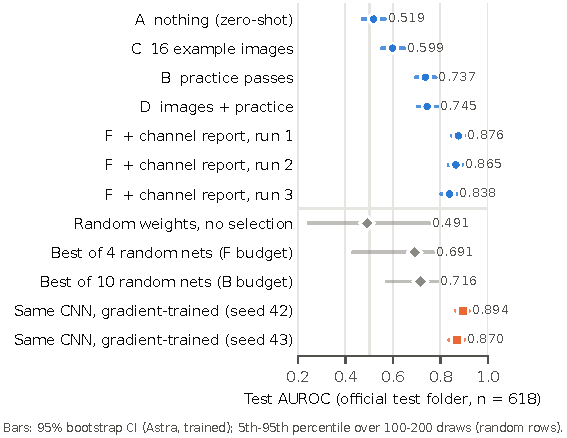
\includegraphics[width=\columnwidth]{project_ladder.pdf}
\caption{Test AUROC by condition. Feedback, not examples, moves the LLM: images alone add 0.08, practice adds 0.22, and the channel report adds a further 0.11. Every F run lies above the 95th percentile of the matched random search and close to gradient training.}
\label{fig:ladder}
\end{figure}

\subsection{Main comparison}
Table~\ref{tab:main} and Fig.~\ref{fig:ladder} answer the research question.
Without feedback, Astra's hand-written network is at chance (A, 0.519), and looking at 16 example images helps little (C, 0.599).
Practice scores are what make it work.
B reaches 0.737, but with 10 evaluations that is not clearly better than the matched random search: 28\,\% of best-of-10 searches score as high.
Adding the images on top of practice changes almost nothing (D, 0.745).
With the channel report, all three independent chats reach 0.838--0.876 (mean 0.859\,$\pm$\,0.016) after only four evaluations each.
Over 100 repetitions, the best-of-4 and best-of-5 searches never exceed 0.821, so every F run beats the matched rival outright.
The gap to gradient training on the same architecture is 0.023 AUROC, and their confidence intervals overlap.
Both trail the pretrained ResNet-50 by about 0.1.
All weight-based methods share the same weakness at $P{=}0.5$: high sensitivity and low specificity, a calibration problem rather than a ranking one.

\subsection{What the LLM actually wrote}
The three F chats began from different first designs: brightness, opacity and texture mixtures at 0.59--0.63 practice AUROC.
In each chat, after the first channel report, Astra noticed that its own \emph{texture} channels (edge magnitude or local intensity range) were consistently higher on normal images.
It rebuilt the readout around them with round-number negative weights, and practice AUROC rose to 0.89--0.93 in the next pass.
Run 3's final network reads a single channel (mean edge magnitude, weight $-1$ per grid cell, bias $+1.25$).
The channel report therefore works as a label-informed \emph{feature-selection} signal: Astra designs a filter bank from domain knowledge, and the report tells it which of its own filters separate the classes.
That is reasoning, not training, but it is not data-free, and we report it as such.
The matched random search also selects on practice labels, but it selects whole networks.
Its winners overfit the practice slices (median practice AUROC 0.84, test 0.69), whereas Astra's F networks keep a smaller gap (practice set 0.93, test 0.86).

\begin{table}[t]
\centering
\caption{Condition G: final layer on a frozen ImageNet ResNet-50 (test $n{=}618$; size-matched subset, 140 images).}
\label{tab:g}
\setlength{\tabcolsep}{2.2pt}
\footnotesize
\begin{tabular}{@{}lcccc@{}}
\toprule
Final layer obtained by & Test AUROC & Spec. & Feat. & Size-matched \\
\midrule
\textbf{Astra, 17 passes + report} & \textbf{0.902} {\scriptsize[0.88, 0.92]} & 0.59 & 26 & 0.724 \\
Selection rule (no LLM) & 0.883 {\scriptsize[0.85, 0.91]} & 0.80 & 32 & 0.669 \\
Best of 17 random heads$^\dagger$ & 0.678 {\scriptsize[0.57, 0.78]} & -- & 2,048 & 0.571 \\
Linear probe, trained & 0.947 {\scriptsize[0.93, 0.96]} & 0.53 & 2,047 & 0.862 \\
\bottomrule
\end{tabular}

\vspace{2pt}
\raggedright\scriptsize $^\dagger$median [5th--95th pct] over 100 repetitions; maximum 0.800. Fit time of the probe: under 1\,s.
\end{table}

\subsection{Stronger features: a frozen ImageNet ResNet-50}\label{sec:g}
Table~\ref{tab:g} repeats the best setting on pretrained features.
Astra used 17 of its 20 passes, changing one thing at a time and comparing passes on overlapping image batches.
Its final layer uses 26 hand-picked features with weights $+4$, $-2$, $\pm1$, $\pm0.5$ and $-0.25$, and bias 0.
It reached 0.902, up from 0.859 on the small CNN.
No random search came close (maximum 0.800), and the mechanical selection rule scored 0.883, so Astra's careful testing added a little beyond ``take the top features''.
The two confidence intervals overlap, however.
The trained linear probe on the same features reached 0.947, a gap of 0.045, twice the gap on the small CNN.
\emph{Explanation, tied to the setup.} With 2,048 unnamed features, an LLM can only shortlist a few dozen that separate on practice images, whereas training uses all of them jointly.
Astra predicted about 0.96, discounting for having consulted the practice set 17 times; practice AUROC ran 0.96--0.98.

\begin{figure}[t]
\centering
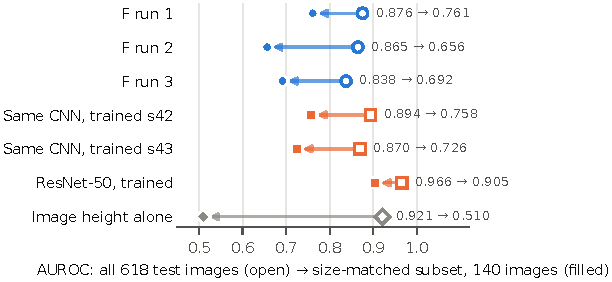
\includegraphics[width=\columnwidth]{project_robust.pdf}
\caption{Robustness check. On 140 test images matched for original width and height, image height alone drops to chance. All models lose AUROC, so part of every score on this dataset comes from acquisition size. Astra's F networks lose more (mean 0.703) than the gradient-trained CNN (0.742). On frozen ImageNet features (G), the trained probe holds (0.862) while hand-selected features fall (Astra 0.724, selection rule 0.669).}
\label{fig:robust}
\end{figure}

\subsection{Robustness: part of the signal is image size}
Fig.~\ref{fig:robust} shows that every model loses AUROC on the size-matched subset.
The F networks drop from 0.859 to 0.703 on average (0.761, 0.656, 0.692; every 95\,\% CI stays above 0.5, lowest bound 0.566).
The same CNN trained by gradient descent drops from 0.882 to 0.742, and ResNet-50 from 0.966 to 0.905.
Within each class, the F2 and F3 scores correlate strongly with log image height (Spearman $\rho$ between $-0.48$ and $-0.72$), as do the trained CNN's ($-0.59$ to $-0.74$).
\emph{Explanation, tied to the data.} Pneumonia files in this dataset are smaller, so after resizing to 224 pixels they show less fine-scale texture.
A rule that scores ``less texture'' as pneumonia therefore reads both the disease (consolidation smooths the lung pattern) and the acquisition size.
Astra found this rule from its channel report, and gradient descent on the same small CNN finds a similar mixture.
Only the larger, ImageNet-pretrained network is largely immune.
This is the shortcut-learning pattern documented for chest X-ray models that pick up hospital and acquisition cues~\cite{zech2018,geirhos2020}.
In all three chats Astra itself warned that the texture cue might reflect acquisition, exposure or processing differences rather than disease.
The same pattern holds on the frozen ResNet-50 features (Table~\ref{tab:g}, Fig.~\ref{fig:robust}).
The trained probe keeps 0.862 on the size-matched subset, but Astra's 26 features fall to 0.724 and the selection rule to 0.669.
Features chosen because they separate the practice images best tend to be the ones that also track image size; a probe that spreads its weight over all 2,048 features is far less exposed.

\subsection{Edit mode: fixing a trained ResNet-50}\label{sec:edit}
In MIT's edit mode, Astra edited the final layer (2,048 weights and a bias) of our trained ResNet-50, given practice feedback from one patient-split half of the test folder (306 images); it was scored on the other half (312 images).
Its edit (mean-centring, pruning small weights, bias $-\ln 2$) left AUROC unchanged (0.954) and raised balanced accuracy from 0.745 to 0.814.
Simply moving the threshold to its best point on the same practice images reached 0.914.
When the only flaw is the operating point, one number fixes it, and an LLM edit adds nothing.

\section{Limitations and future work}
We used one LLM and one dataset.
F has three chats, and each other condition has one.
G has one chat.
The loop was run by hand, which caused one log reset (F run 1) and one accidental re-run (F run 3); both are documented, and neither gave Astra extra information.
In G, Astra was allowed a tool only to read the long reports (all 36 commands were plain file reads), and it read the top and bottom of each report, so our sort order shaped its shortlist.
The size-matched subset is small (140 images) and atypical (large pneumonia and small normal files), so absolute AUROC there is lower for every model.
The comparison between models matters more than the level.
Astra's compute cannot be measured, so ``time'' is human wall-clock.
A longer study would automate the loop, add a second LLM, normalise acquisition size in preprocessing before the LLM sees any feedback, test on an external pediatric collection, and give the LLM a report on feature \emph{groups} rather than 2,048 single features, so that it can use more of the representation.

\section*{AI-use statement and contributions}
\emph{AI use.} GPT-6 Astra is the system under study.
Every prompt, transcript, weight file and practice log is in the repository~\cite{repo}.
Claude (Anthropic) was used as a coding and writing assistant.
It wrote the pipeline extensions (practice runner, channel report, static checks, random-search baselines, robustness check, figures) and drafted this report from our results.
The group ran every experiment in Google Colab, ran the Astra chats, checked the transcripts, and is responsible for all numbers, which come from our own runs.
\emph{Contributions.} Mahd Hindi: [to be completed]. Khaled AlHassani: [to be completed]. Abdulla AlKaabi: [to be completed].

\begin{thebibliography}{6}
\footnotesize
\bibitem{takehi2026} R.~Takehi, J.~Teoh, A.~Zhang and O.~Khattab, ``Sparks of weight-space programming: LLMs can natively read \& write neural network weights,'' MIT CSAIL blog post (not peer-reviewed), Nov.~2026. [Online]. Available: \url{https://rikiyat.github.io/blog/weight-space-programming/}
\bibitem{kermany2018} D.~S.~Kermany \emph{et al.}, ``Identifying medical diagnoses and treatable diseases by image-based deep learning,'' \emph{Cell}, vol.~172, no.~5, pp.~1122--1131, 2018.
\bibitem{singh2024} S.~Singh \emph{et al.}, ``Efficient pneumonia detection using Vision Transformers on chest X-rays,'' \emph{Scientific Reports}, vol.~14, art.~2487, 2024.
\bibitem{geirhos2020} R.~Geirhos \emph{et al.}, ``Shortcut learning in deep neural networks,'' \emph{Nature Machine Intelligence}, vol.~2, pp.~665--673, 2020.
\bibitem{zech2018} J.~R.~Zech \emph{et al.}, ``Variable generalization performance of a deep learning model to detect pneumonia in chest radiographs,'' \emph{PLOS Medicine}, vol.~15, no.~11, e1002683, 2018.
\bibitem{repo} M.~Hindi, K.~AlHassani and A.~AlKaabi, code, prompts, transcripts and results. [Online]. Available: \url{https://github.com/mahdhindi/pneumonia-cxr-algorithm-comparison} (branch \texttt{a2-paper-critique}).
\end{thebibliography}

\end{document}
